\documentclass{sintefbeamer}
\usepackage[UTF8]{ctex}
\usepackage{subcaption}
\usepackage{hyperref}
\usepackage{tcolorbox}


% meta-data
\title{极限飞盘协会成立答辩}
% \subtitle{推动校园体育文化发展}
\author{极限飞盘协会筹备组}
\date{\today}
\titlebackground{images/background}

% document body
\begin{document}

\maketitle

\section{社团基本情况}

\begin{frame}{社团概况}{\thesection \, \secname}
  \begin{itemize}
    \item \textbf{社团名称}:哈尔滨工业大学(深圳)极限飞盘协会
    \item \textbf{英文名}:Association of Ultimate Frisbee, Harbin Institute of Technology, Shenzhen
    \item \textbf{指导老师}:火栋,未来学部经济管理学院教师
    \item \textbf{指导单位}:未来学部
    % \item \textbf{定位}:以极限飞盘运动为核心,集体育锻炼、团队协作、文化推广于一体的综合性学生社团。
    % \item \textbf{宗旨}:推广极限飞盘运动,提升学生身体素质和团队合作能力,丰富校园文化生活。
  \end{itemize}
  
  % \vspace{4em}
  
  \begin{columns}[T]
    \begin{column}{0.48\textwidth}
      \fcolorbox{sintefblue}{white}{
        \parbox[t][2cm]{\dimexpr\linewidth-2\fboxsep-2\fboxrule}{
          \textbf{\textcolor{sintefblue}{定位}}\\[0.5em]
          以极限飞盘运动为核心,集体育锻炼、团队协作、文化推广于一体的综合性学生社团。
        }
      }
    \end{column}
    \hfill
    \begin{column}{0.48\textwidth}
      \fcolorbox{sintefblue}{white}{
        \parbox[t][2cm]{\dimexpr\linewidth-2\fboxsep-2\fboxrule}{
          \textbf{\textcolor{sintefblue}{宗旨}}\\[0.5em]
          推广极限飞盘运动,提升学生身体素质和团队合作能力,丰富校园文化生活。
        }
      }
    \end{column}
  \end{columns}
\end{frame}

\begin{frame}{组织架构与核心成员}{\thesection \, \secname}

  \begin{columns}[T]
    \begin{column}{0.5\textwidth}
      \begin{center}
        {\huge\textbf{\textcolor{sintefblue}{社团架构}}}
      \end{center}
      % \vspace{0.5em}
      \begin{center}
        \includegraphics[height=0.8\textheight, keepaspectratio]{./images/未命名绘图.drawio.png}
      \end{center}
    \end{column}

    \hspace{-1.5em}{\color{sintefblue}\vrule width 1pt}\hspace{1.2em}

    \begin{column}{0.5\textwidth}
      % \begin{center}
      %   \includegraphics[trim=0 0 0 3.2cm, clip, width=0.95\textheight, keepaspectratio]{./images/核心成员名单.pdf}
      % \end{center}
      \begin{center}
        {\huge\textbf{\textcolor{sintefblue}{核心力量}}}
      \end{center}
      \vspace{0.5em}
      \parbox{\linewidth}{
      \textcolor{sintefblue}{核心团队}\\
      由15位来自不同学部、年级的本硕博同学组成,涵盖管理、训练、赛事组织、宣传等多个职能部门。
      \\
      \\
      \textcolor{sintefblue}{成员构成}\\
      覆盖全校各大学部,促进跨学科交流
      }
    \end{column}

  \end{columns}

  
\end{frame}

% \begin{frame}{核心成员介绍}{\thesection \, \secname}
  
% \end{frame}

\begin{frame}{社团旗帜与徽章}{\thesection \, \secname}
 \begin{columns}
  \begin{column}{0.5\textwidth}
    \begin{figure}
      \centering
      \includegraphics[width=\textwidth]{./images/协会徽章旗帜_部分1.pdf}
      \caption{协会徽章}
    \end{figure}
  \end{column}
  \begin{column}{0.5\textwidth}
    \begin{figure}
      \centering
      \includegraphics[width=\textwidth]{./images/协会徽章旗帜_部分3.pdf}
      \caption{协会旗帜}
    \end{figure}
  \end{column}
\end{columns}
\end{frame}

% \begin{frame}{社团旗帜与徽章}{\thesection \, \secname}
%  \begin{columns}
%   \begin{column}{0.5\textwidth}
%     \begin{figure}
%       \centering
%       \includegraphics[width=\textwidth]{./images/协会徽章旗帜_部分3.pdf}
%       \caption{协会旗帜1}
%     \end{figure}
%   \end{column}
%   \begin{column}{0.5\textwidth}
%     \begin{figure}
%       \centering
%       \includegraphics[width=\textwidth]{./images/协会徽章旗帜_部分4.pdf}
%       \caption{协会旗帜2}
%     \end{figure}
%   \end{column}
% \end{columns}
% \end{frame}

\begin{frame}{社员人数}{\thesection \, \secname}

  \begin{columns}[onlytextwidth]
    \begin{column}{0.4\textwidth}
      \parbox{\dimexpr\linewidth-2\fboxsep-2\fboxrule}{
      
      \textbf{\textcolor{sintefblue}{\fontsize{45pt}{54pt}\selectfont 60+}}
      
      次日常活动\\
      
      \textbf{\textcolor{sintefblue}{\fontsize{45pt}{54pt}\selectfont 500+}}
      
      成员社群基础(QQ与微信)\\
      
      \textbf{\textcolor{sintefblue}{\fontsize{45pt}{54pt}\selectfont 70+}}
      
      高度活跃成员
    }
    \end{column}

    \begin{column}{0.6\textwidth}
      
      \parbox{\dimexpr\linewidth-2\fboxsep-2\fboxrule}{
      \begin{figure}
        \centering
        \includegraphics[height=\textheight, keepaspectratio]{./images/群聊.png}
      \end{figure}
    }
      
    \end{column}
  \end{columns}

   
  % QQ群386人,微信群423人、257人,高度活跃人数为72人。
  % \begin{center}
  %   \includegraphics[width=0.25\textwidth,height=0.8\textheight, keepaspectratio]{./images/qq.png}
  %   \includegraphics[width=0.25\textwidth,height=0.8\textheight, keepaspectratio]{./images/wx1.png}
  %   \includegraphics[width=0.25\textwidth,height=0.8\textheight, keepaspectratio]{./images/wx2.png}
  %   \includegraphics[width=0.25\textwidth,height=0.8\textheight, keepaspectratio]{./images/wx3.png}
  % \end{center}
\end{frame}

\section{社团成立的目的和意义}

% \begin{frame}{极限飞盘是什么}{\thesection \, \secname}
%   \begin{itemize}
%     \item 极限飞盘是7v7的男女混合(4男3女或3男4女)无身体对抗的团队运动,以传接技巧和团队的配合为主,比赛过程中大量的跑动对身体素质提出了较高要求。
%     \item 两队轮流进攻防守,进攻方通过传接飞盘向对方得分区推进,防守方则通过阻挡传接线路或抢断飞盘来阻止对方得分。每次成功在得分区内接到飞盘得1分,比赛时间结束时得分高的一方获胜。
%     \item 极限飞盘强调“飞盘精神”(Spirit of the Game),比赛过程中无裁判,运动员需自我裁决,培养自律与诚信。
%   \end{itemize}
% \end{frame}

\begin{frame}{极限飞盘是什么}{\thesection \, \secname}
  \begin{columns}[T]
    \begin{column}{0.3\textwidth}
      \centering
      \textbf{\textcolor{sintefblue}{融合多种运动的快节奏对抗}}\\
      结合了橄榄球的跑动、足球的战术和篮球的传切,充满速度与激情
    \end{column}
    \begin{column}{0.3\textwidth}
      \centering
      \textbf{\textcolor{sintefblue}{独特的“飞盘精神”}}\\
      ~\\
      一项自我裁判的运动,强调公平竞争、相互尊重和享受比赛的乐趣
    \end{column}
    \begin{column}{0.3\textwidth}
      \centering
      \textbf{\textcolor{sintefblue}{零身体接触的安全运动}}\\
      ~\\
      规则禁止身体冲撞,鼓励技术与智慧的较量
    \end{column}
  \end{columns}

  \vspace{0.5em}

  \begin{columns}[b]
    \begin{column}{0.3\textwidth}
      \begin{figure}
        \centering
        \includegraphics[width=\textwidth]{./images/争夺一个盘.png}
      \end{figure}
    \end{column}
    \begin{column}{0.3\textwidth}
      \begin{figure}
        \centering
        \includegraphics[width=\textwidth]{./images/circle.jpg}
      \end{figure}
    \end{column}
    \begin{column}{0.3\textwidth}
      \begin{figure}
        \centering
        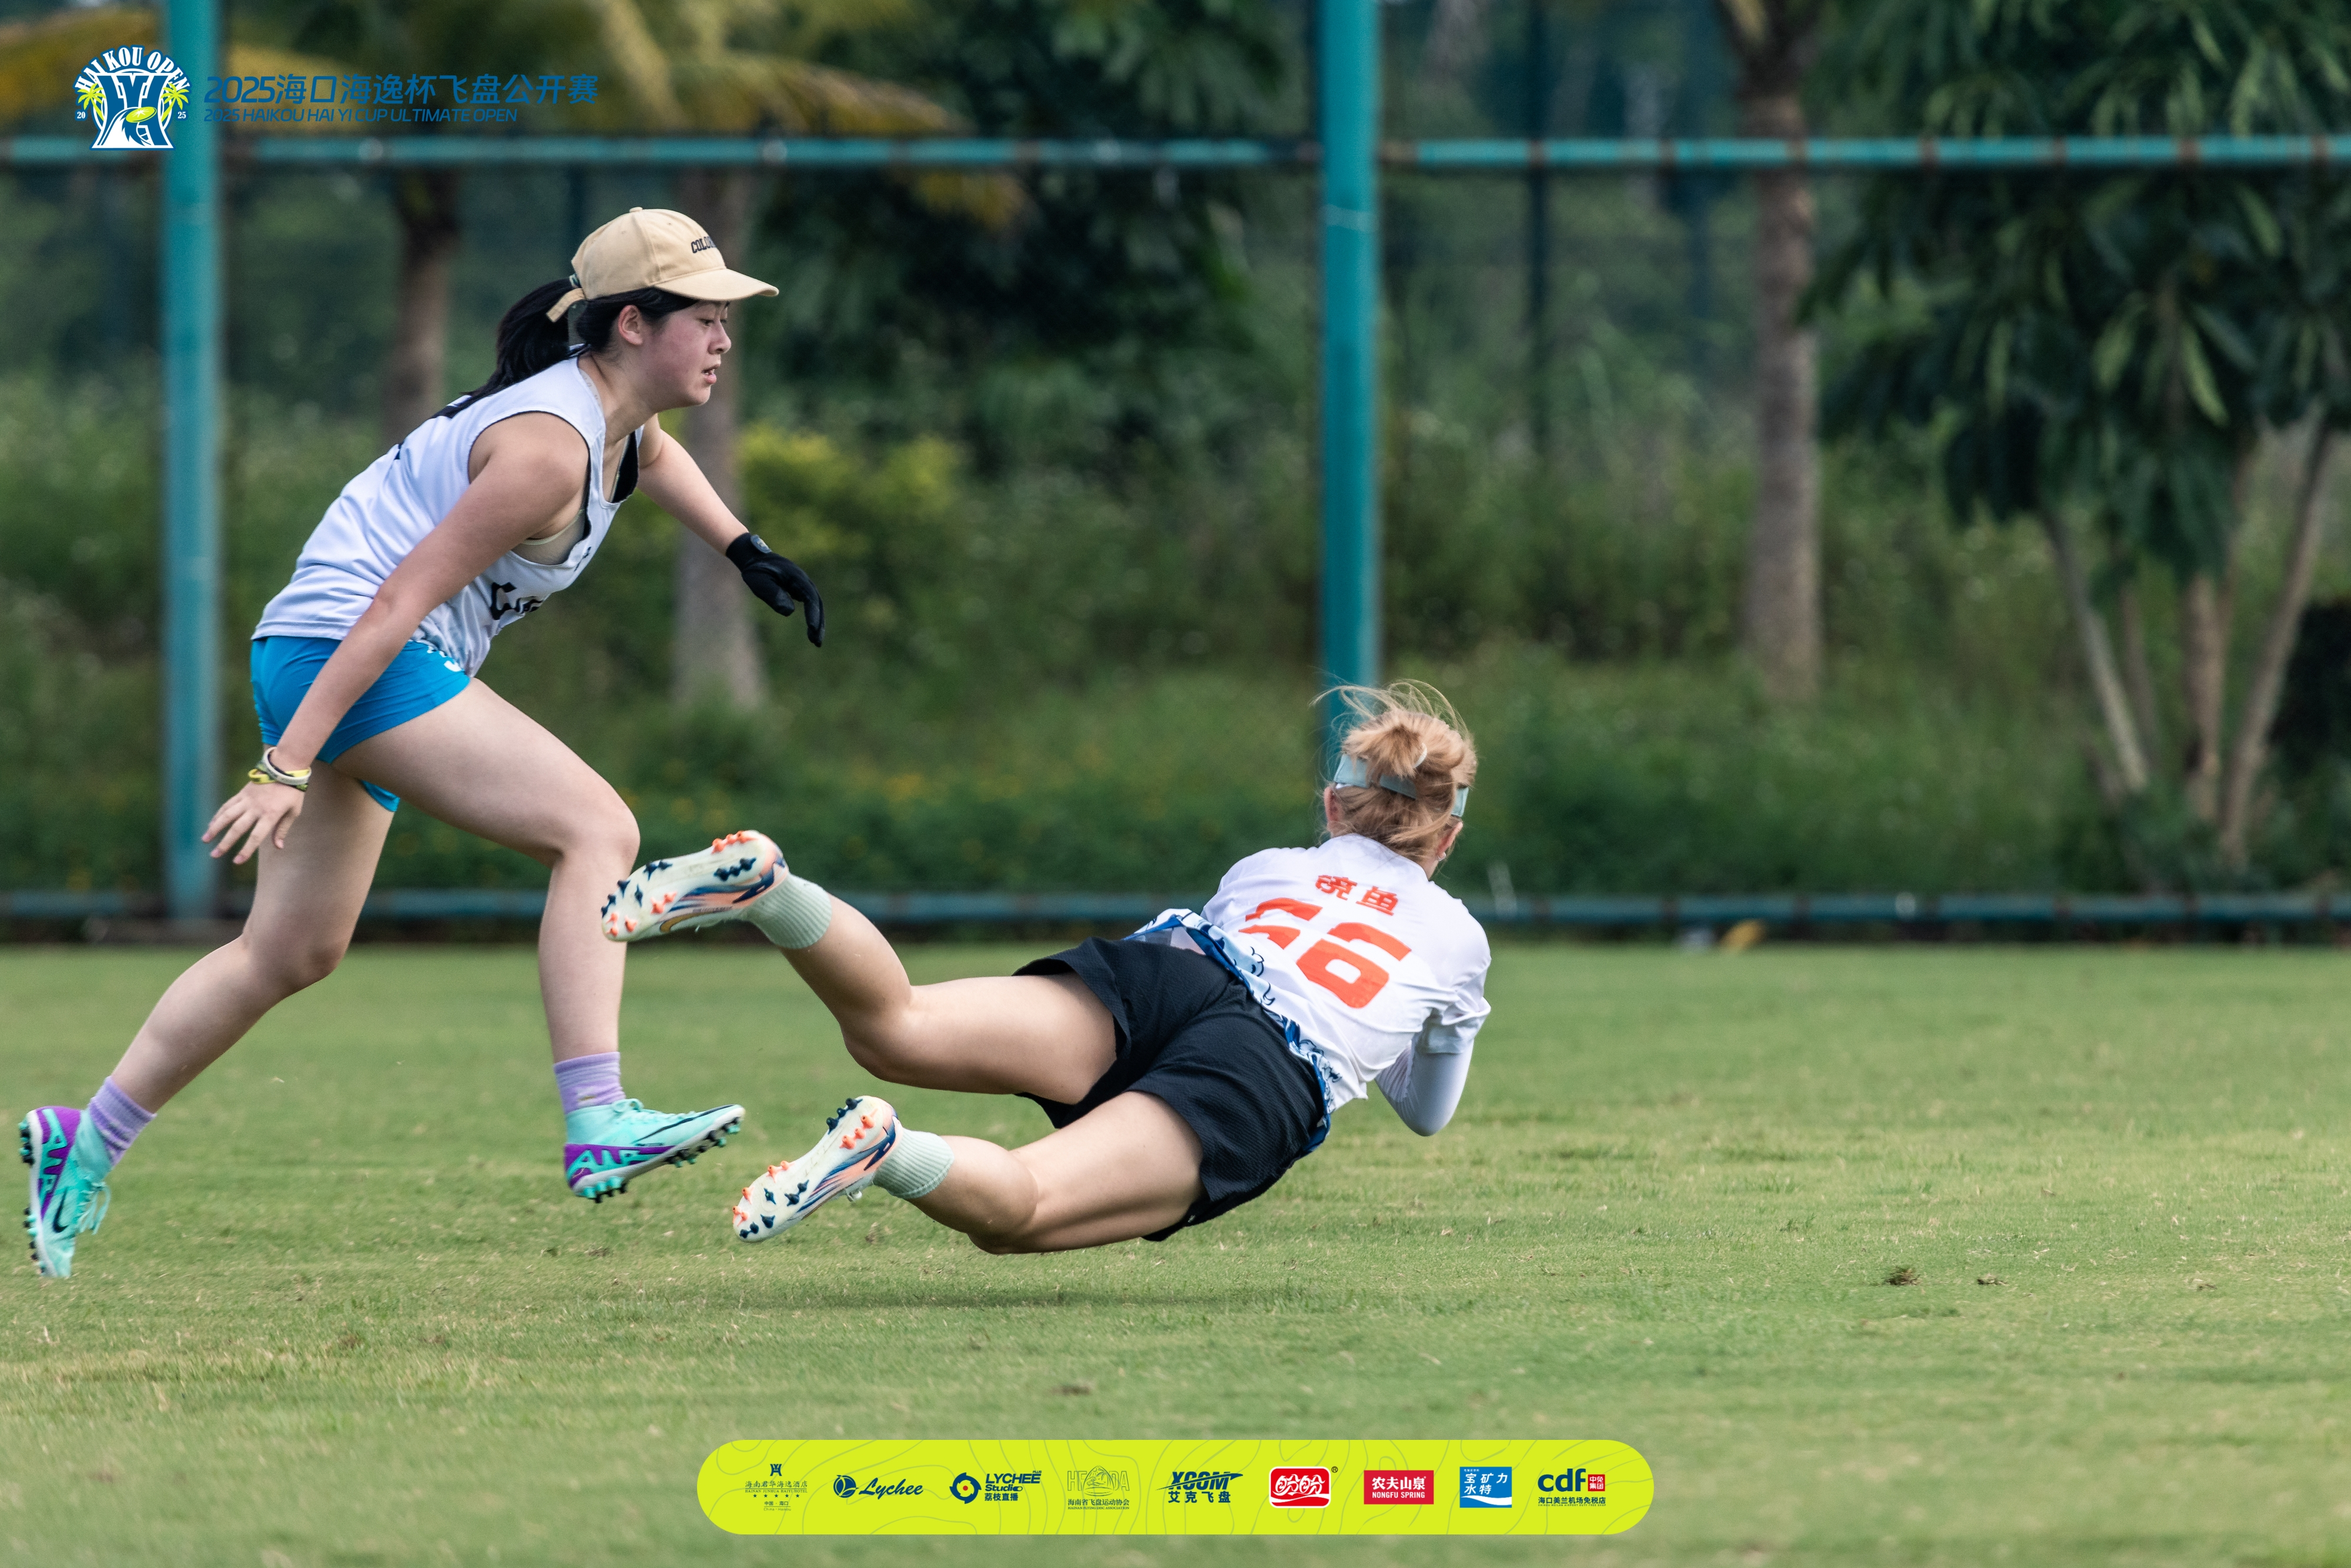
\includegraphics[width=\textwidth]{./images/yjy.jpg}
      \end{figure}
    \end{column}
  \end{columns}
\end{frame}

% \begin{frame}{飞盘场地}{\thesection \, \secname}
%   \begin{center}
%     \includegraphics[width=0.555\textwidth, height=0.8\textheight, keepaspectratio]{./images/场地1.png}
%     \includegraphics[width=0.55\textwidth, height=0.8\textheight, keepaspectratio]{./images/场地2.png}
%   \end{center}
% \end{frame}
\begin{frame}{团队飞盘目前发展}{\thesection \, \secname}
  \begin{columns}[T]
    \begin{column}{0.32\textwidth}
      \begin{block}{\textbf{\textcolor{sintefblue}{教育部官方纳入}}}
        {\color{sintefblue}\rule{\linewidth}{1pt}}
        在教育部印发的《义务教育课程方案和课程标准》中,“极限飞盘”入选"体育与健康课程标准"板块
        
        \begin{tcolorbox}[height=1.8cm, valign=center, colback=sintefblue!10, colframe=sintefblue, sharp corners]
          \begin{center}
            \textbf{\textcolor{sintefblue}{正式列入义务教育阶段课程}}
          \end{center}
        \end{tcolorbox}
      \end{block}
    \end{column}
    \hfill
    \begin{column}{0.32\textwidth}
      \begin{block}{\textbf{\textcolor{sintefblue}{体育总局全力推动}}}
        {\color{sintefblue}\rule{\linewidth}{1pt}}
        国家体育总局社体中心举办中国飞盘联赛,2024年起同步纳入全民健身赛事活动框架
        
        \begin{tcolorbox}[height=1.8cm, valign=center, colback=sintefblue!10, colframe=sintefblue, sharp corners]
          \begin{center}
            \textbf{\textcolor{sintefblue}{纳入全民健身赛事活动框架}}
          \end{center}
        \end{tcolorbox}
      \end{block}
    \end{column}
    \hfill
    \begin{column}{0.32\textwidth}
      \begin{block}{\textbf{\textcolor{sintefblue}{团队飞盘入选世运会}}}
        {\color{sintefblue}\rule{\linewidth}{1pt}}
        在第6届日本秋田世运会上,飞盘(包括团队飞盘和掷准飞盘)正式成为奖牌项目
        
        \begin{tcolorbox}[height=1.8cm, valign=center, colback=sintefblue!10, colframe=sintefblue, sharp corners]
          \begin{center}
            \textbf{\textcolor{sintefblue}{2025年成都世运会,项目收获了大量关注}}
          \end{center}
        \end{tcolorbox}
      \end{block}
    \end{column}
  \end{columns}
\end{frame}


% 中国大学生极限飞盘联盟(Chinese University Ultimate Association,简称CUUA)是由乐奥体育CEO王念飞发起,2014年联合中国高校极限飞盘协会成立的非营利性学生主导赛事组织,旨在推广飞盘运动、提升竞技水平并传承“尊重、诚信、团队”的飞盘精神 [2-3]。联盟赛事体系包含预选赛、地区赛和全国总决赛三级架构,2025年第七届赛事覆盖全国146支队伍(含124支学校队伍),设置11场预选赛与4场地区赛 [2] [4-5]。
% 截至2025年,联盟成员已扩展至全国60余所高校 [3] [6]。赛事由高校队伍通过地区赛晋级,如第七届南部地区赛吸引广东工业大学、中山大学等10所高校参赛,华中科技大学队在第七届华中地区预选赛中首次获得季军 [1] [6]。

\begin{frame}{社团成立意义}{\thesection \, \secname}
  \begin{columns}[T]
    \begin{column}{0.48\textwidth}
      \begin{block}{填补校园体育空白}
        \small 引入新兴时尚运动,填补校内空白,提供区别于传统球类的新颖选择
      \end{block}
      \begin{block}{强健体魄与培养习惯}
        \small 通过趣味性强的户外运动促进学生体育锻炼,培养良好运动习惯
      \end{block}
      \begin{block}{提升团队协作与领导力}
        \small 强调团队配合,在战术讨论和场上指挥中锻炼沟通与领导能力
      \end{block}
    \end{column}
    
    \begin{column}{0.48\textwidth}
      \begin{block}{践行独特“飞盘精神”}
        \small 坚持无裁判、自我裁决规则,培养自律、诚信与相互尊重的品格
      \end{block}
      \begin{block}{促进跨界交流融合}
        \small 搭建跨院系、跨年级的社交平台,营造充满活力的青春校园氛围
      \end{block}
      \begin{block}{响应号召展示形象}
        \small 贯彻“全民健身”理念,参加比赛提升学校知名度,展示学子风采
      \end{block}
    \end{column}
  \end{columns}
\end{frame}

\section{社团成立筹备工作情况}

\begin{frame}{日常活动}{\thesection \, \secname}
  \begin{center}
    \includegraphics[width=0.9\textwidth]{./images/报名接龙.png}
  \end{center}
  \vspace{-0.9em}
  \begin{center}
    \textbf{\textcolor{sintefblue}{\fontsize{45pt}{54pt}\selectfont 60+}}次日常活动,涵盖训练、教学、友谊赛等多种形式
  \end{center}
\end{frame}

\begin{frame}{日常活动}{\thesection \, \secname}
  
  \vspace{0.5em}
  \begin{center}
    \includegraphics[width=\textwidth, keepaspectratio]{./images/组图4.pdf}
  \end{center}
  \vspace{0.3em}
  \begin{center}
    涵盖\textbf{\textcolor{sintefblue}{\fontsize{20pt}{24pt}\selectfont 训练}}、\textbf{\textcolor{sintefblue}{\fontsize{20pt}{24pt}\selectfont 教学}}、\textbf{\textcolor{sintefblue}{\fontsize{20pt}{24pt}\selectfont 友谊赛}}等多种形式
  \end{center}
\end{frame}

\begin{frame}{日常活动}{\thesection \, \secname}

  \begin{columns}
    \begin{column}{0.3\textwidth}
      
      \begin{block}{\textbf{\textcolor{sintefblue}{大学城三校训练}}}
        {\color{sintefblue}\rule{\linewidth}{1pt}}
        目前深圳大学城清华大学、北京大学均成立了飞盘协会,哈工大同学与其他两个学校协会的同学交流密切,目前已有40余位同学长期训练,每周定期组织协会活动。
      \end{block}
    \end{column}

    \begin{column}{0.7\textwidth}
      \begin{figure}
        \centering
        \includegraphics[width=\textwidth, keepaspectratio]{./images/大学城1.pdf}
        \caption{大学城三校训练}
      \end{figure}
    \end{column}
  \end{columns}

\end{frame}

% \begin{frame}{日常活动}{\thesection \, \secname}

%   \begin{center}
%     \includegraphics[height=\textheight, keepaspectratio]{./images/大学城.jpg}
%   \end{center}

% \end{frame}

% \begin{frame}{校内品牌赛事}{\thesection \, \secname}
%   \begin{itemize}
%     \item 协会运行至今已举办4场大型的校级极限飞盘赛事:
%     \item \textbf{2024体育文化节极限飞盘赛}
%     \item \textbf{2024新生杯极限飞盘赛(美碳杯)}
%     \item \textbf{2025体育文化节极限飞盘赛(盘不落地,永不放弃)}
%     \item \textbf{2025新生杯极限飞盘赛}
%     \item 获得了头部飞盘运动品牌翼鲲飞盘的赞助,总计吸引了包括留学生在内的来自全校不同专业、年级的200余位同学参与,极大地丰富了同学们的文体生活。
%   \end{itemize}
% \end{frame}

\begin{frame}{校内品牌赛事}{\thesection \, \secname}
  % \begin{itemize}
  %   \item 协会运行至今已举办4场大型的校级极限飞盘赛事:
  %   \item \textbf{2024体育文化节极限飞盘赛}
  %   \item \textbf{2024新生杯极限飞盘赛(美碳杯)}
  %   \item \textbf{2025体育文化节极限飞盘赛(盘不落地,永不放弃)}
  %   \item \textbf{2025新生杯极限飞盘赛}
  %   \item 获得了头部飞盘运动品牌翼鲲飞盘的赞助,总计吸引了包括留学生在内的来自全校不同专业、年级的200余位同学参与,极大地丰富了同学们的文体生活。
  % \end{itemize}

  \begin{center}
    \includegraphics[height=0.9\textheight, keepaspectratio]{./images/组图合照.pdf}
  \end{center}
  \begin{center}
      2024\&2025新生杯极限飞盘赛,2024\&2025体育文化节极限飞盘赛\\
      累计吸引\textbf{\textcolor{sintefblue}{\fontsize{20pt}{24pt}\selectfont 200+}}来自全校各年级、专业的同学参与,广受好评。
  \end{center}

\end{frame}

% \begin{frame}{2024体育文化节极限飞盘赛}{\thesection \, \secname}
%   \begin{columns}
%   \begin{column}{0.25\textwidth}
%     \begin{figure}
%       \centering
%       \includegraphics[width=\textwidth]{./images/2024体育文化节海报.jpg}
%       \caption{2024体育文化节}
%     \end{figure}
%   \end{column}
%   \begin{column}{0.65\textwidth}
%     \begin{figure}
%       \centering
%       \includegraphics[width=\textwidth]{./images/工大赛事8.JPG}
%       \caption{2024体育文化节极限飞盘赛}
%     \end{figure}
%   \end{column}
% \end{columns}
% \end{frame}

% \begin{frame}{2024新生杯极限飞盘赛}{\thesection \, \secname}
%   \begin{columns}
%   \begin{column}{0.22\textwidth}
%     \begin{figure}
%       \centering
%       \includegraphics[width=\textwidth]{./images/2024新生杯海报.jpg}
%       \caption{2024新生杯}
%     \end{figure}
%   \end{column}
%   \begin{column}{0.78\textwidth}
%     \begin{figure}
%       \centering
%       \includegraphics[width=0.9\textwidth]{./images/工大赛事4.jpg}
%       \caption{2024新生杯极限飞盘赛}
%     \end{figure}
%   \end{column}
% \end{columns}
% \end{frame}

% \begin{frame}{2025体育文化节极限飞盘赛}{\thesection \, \secname}
%   \begin{columns}
%   \begin{column}{0.3\textwidth}
%     \begin{figure}
%       \centering
%       \includegraphics[width=\textwidth]{./images/2025体育文化节海报.jpg}
%       \caption{2025体育文化节}
%     \end{figure}
%   \end{column}
%   \begin{column}{0.7\textwidth}
%     \begin{figure}
%       \centering
%       \includegraphics[width=\textwidth]{./images/2025体育文化节大合照.jpg}
%       \caption{2025体育文化节极限飞盘赛}
%     \end{figure}
%   \end{column}
% \end{columns}
% \end{frame}

% \begin{frame}{2025新生杯极限飞盘赛}{\thesection \, \secname}
%   \begin{columns}
%   \begin{column}{0.28\textwidth}
%     \begin{figure}
%       \centering
%       \includegraphics[width=\textwidth]{./images/2025新生杯海报.jpg}
%       \caption{2025新生杯}
%     \end{figure}
%   \end{column}
%   \begin{column}{0.72\textwidth}
%     \begin{figure}
%       \centering
%       \includegraphics[width=\textwidth]{./images/2025新生杯大合照.jpg}
%       \caption{2025新生杯极限飞盘赛}
%     \end{figure}
%   \end{column}
% \end{columns}
% \end{frame}

% \begin{frame}{校际交流赛}{\thesection \, \secname}
%   与南方科技大学、深圳大学、深圳技术大学等高校飞盘协会多次交流切磋,提升了协会整体水平。
%   \begin{columns}
%   \begin{column}{0.5\textwidth}
%     \begin{figure}
%       \centering
%       \includegraphics[width=\textwidth]{./images/南科大2.png}
%       \caption{南方科技大学1}
%     \end{figure}
%   \end{column}
%   \begin{column}{0.5\textwidth}
%     \begin{figure}
%       \centering
%       \includegraphics[width=\textwidth]{./images/南科大.jpg}
%       \caption{南方科技大学2}
%     \end{figure}
%   \end{column}
% \end{columns}
% \end{frame}

% \begin{frame}{校际交流赛}{\thesection \, \secname}
%   \begin{columns}
%   \begin{column}{0.5\textwidth}
%     \begin{figure}
%       \centering
%       \includegraphics[width=\textwidth]{./images/深大.jpg}
%       \caption{深圳大学}
%     \end{figure}
%   \end{column}
%   \begin{column}{0.5\textwidth}
%     \begin{figure}
%       \centering
%       \includegraphics[width=\textwidth]{./images/港中深.jpg}
%       \caption{香港中文大学(深圳)}
%     \end{figure}
%   \end{column}
% \end{columns}
% \end{frame}
\begin{frame}{校际交流赛}{\thesection \, \secname}
  \begin{center}
    \includegraphics[height=0.98\textheight, keepaspectratio]{./images/校际1.pdf}
  \end{center}
  \begin{center}
    与南科大、深大、深技大、港中深等高校飞盘协会多次交流切磋
  \end{center}
\end{frame}

\begin{frame}{湾区交流赛}{\thesection \, \secname}
  \begin{center}
    \includegraphics[width=0.95\textwidth]{./images/湾区交流赛2.pdf}
  \end{center}

  \begin{itemize}
    \item 2024年11月23日,北京大学组织首届“湾区高校青年飞盘邀请赛”,邀请包括清华大学、哈尔滨工业大学(深圳)、香港大学、深圳大学、南方科技大学、深圳技术大学、香港中文大学(深圳)在内等多所高校参赛,吸引了超过100名选手参与。
    \item 2025年10月31日,第二届“湾区高校青年飞盘邀请赛”
  \end{itemize}

\end{frame}

% \begin{frame}{湾区交流赛}{\thesection \, \secname}
%   \begin{columns}
%   \begin{column}{0.5\textwidth}
%     \begin{figure}
%       \centering
%       \includegraphics[width=\textwidth]{./images/第一届湾区1.jpg}
%       \caption{第一届湾区交流赛}
%     \end{figure}
%   \end{column}
%   \begin{column}{0.5\textwidth}
%     \begin{figure}
%       \centering
%       \includegraphics[width=\textwidth]{./images/第二届湾区.jpg}
%       \caption{第二届湾区交流赛}
%     \end{figure}
%   \end{column}
% \end{columns}
% \end{frame}

\begin{frame}{“深爱人才,圳在运动”\\全球名校人才体育风尚季飞盘赛}{\thesection \, \secname}
  2025年9月13日,“深爱人才 圳在运动”全球名校人才体育风尚季飞盘赛在深圳市罗湖区仙桐体育公园激情开赛。哈尔滨工业大学深圳校区校友代表队凭借出色发挥,不仅以小组赛第一的身份晋级,更在全程五场赛事中取得四胜的亮眼战绩,充分展现了哈工大人的卓越竞技风采与精神风貌。
\end{frame}

\begin{frame}{“深爱人才,圳在运动”\\全球名校人才体育风尚季飞盘赛}{\thesection \, \secname}
  \begin{center}
    \includegraphics[height=0.95\textheight, keepaspectratio]{./images/深爱人才.jpg}
  \end{center}
  \begin{center}
    哈尔滨工业大学深圳校区校友代表队凭借出色发挥,不仅以小组赛第一的身份晋级,更在全程五场赛事中取得四胜的亮眼战绩,充分展现了哈工大人的卓越竞技风采与精神风貌。
    
  \end{center}
\end{frame}

\begin{frame}{未来展望}{\thesection \, \secname}
  \begin{itemize}
    \item 计划建立极限飞盘校队,备战今年3月的全国大学生极限飞盘联赛预选赛,争取为学校赢得荣誉。
  \end{itemize}
  \begin{center}
    \includegraphics[height=\textheight, keepaspectratio]{./images/cuua.jpg}
  \end{center}
\end{frame}

\begin{frame}{宣传推广}{\thesection \, \secname}
  \begin{itemize}
    \item 组织飞盘比赛观赛活动,设计赛事纪念小飞盘,提升同学们对飞盘运动的兴趣。
    \item 组织战术讲解与观赛活动,提升同学们对飞盘运动的理解。
    \item 设计并制作队服,增强团队凝聚力。
  \end{itemize}
  
  \begin{center}
    \includegraphics[height=0.9\textheight, keepaspectratio]{./images/观赛.jpg}
  \end{center}
\end{frame}

\begin{frame}{宣传推广}{\thesection \, \secname}
  \begin{columns}
  \begin{column}{0.5\textwidth}
    \begin{figure}
      \centering
      \includegraphics[width=\textwidth]{./images/mini.jpg}
      \caption{纪念小飞盘}
    \end{figure}
  \end{column}
  \begin{column}{0.4\textwidth}
    \begin{figure}
      \centering
      \includegraphics[height=0.9\textheight]{./images/战术.jpg}
      \caption{战术讲解}
    \end{figure}
  \end{column}
\end{columns}
\end{frame}

\begin{frame}{宣传推广}{\thesection \, \secname}
  \begin{columns}
  \begin{column}{0.5\textwidth}
    \begin{figure}
      \centering
      \includegraphics[height=0.9\textheight]{./images/白色队服.jpg}
      \caption{白色队服}
    \end{figure}
  \end{column}
  \begin{column}{0.5\textwidth}
    \begin{figure}
      \centering
      \includegraphics[height=0.9\textheight]{./images/蓝色队服.jpg}
      \caption{蓝色队服}
    \end{figure}
  \end{column}
\end{columns}
\end{frame}

\begin{frame}{宣传推广}{\thesection \, \secname}
  \begin{itemize}
    \item \textbf{线上宣传}:
      \begin{itemize}
        \item 建立微信公众号、抖音等新媒体平台,建立本校\href{https://hitsz-frisbee.top}{极限飞盘协会网站}
        \item 制作\href{https://www.bilibili.com/video/BV1oNLVznEKZ/}{宣传视频}和海报
      \end{itemize}
    \item \textbf{线下推广}:
      \begin{itemize}
        \item 百团大战宣传
        \item 游园会宣传
      \end{itemize}
    \item \textbf{品牌建设}:设计协会LOGO、口号和队服
  \end{itemize}
\end{frame}

\begin{frame}{资源保障}{\thesection \, \secname}
  \begin{itemize}
    \item 经费来源:不收取会费,物资由校团委经费支持和企业赞助提供。
    \item 器材配置:飞盘*10,训练角标*20,标志锥*4,急救包*1。
  \end{itemize}
\end{frame}

\begin{frame}{风险评估与应对}{\thesection \, \secname}
  \begin{itemize}
    \item 安全保障:运动保险、应急预案、急救药箱
    \item 可持续发展:梯队培养、档案管理、经验传承
    \item 财务监管:财务公示、接受监督
  \end{itemize}
\end{frame}

\backmatter

\end{document}
